\chapter{The HH$\rightarrow$4b analysis at ATLAS}

The search for the exact shape of the Higgs potential is an interesting endeavor as its not only  directly related to \ac{ewsb} but also could solve some fundamental questions about the nature of the universe as described in section \ref{sec:beyond_sm}. Since the Higgs interacts via Yukawa couplings from equation \ref{eq:yukawa_term} the coupling strengths for fermions are directly proportional to their mass and thus the Higgs couples most strongly to heavy particles. The main production modes at the \ac{lhc} are shown in figure \ref{fig:main_production_processes}. All couplings in the following are scaled with respect to their \ac{sm} values and are denoted with $\kappa_\mathrm{c} = c/c_\mathrm{sm}$ so that $\kappa_\mathrm{c}=1$ represents the \ac{sm} value of some coupling $c$.

\begin{figure}
    \centering
    \subfigure[]{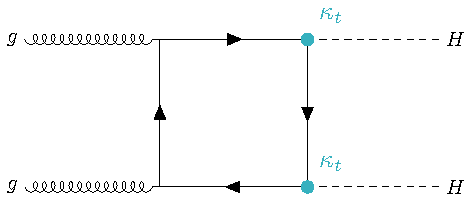
\includegraphics[width=.42\textwidth]{fig_01a}}\hspace{.06\textwidth}
    \subfigure[]{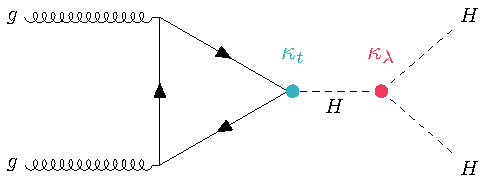
\includegraphics[width=.42\textwidth]{fig_01b}} \\
    \subfigure[]{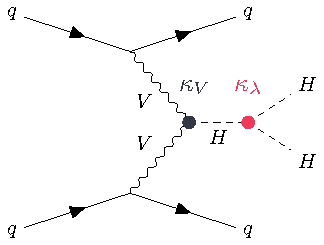
\includegraphics[width=.3\textwidth]{fig_02a}}\hspace{.01\textwidth}
    \subfigure[]{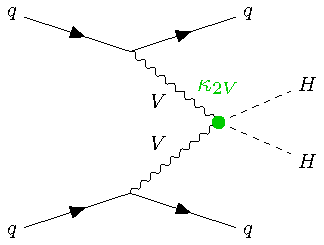
\includegraphics[width=.3\textwidth]{fig_02b}}\hspace{.01\textwidth}
    \subfigure[]{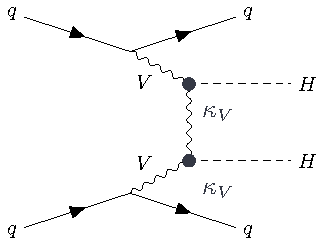
\includegraphics[width=.3\textwidth]{fig_02c}}
    \caption[]{Leading Higgs Pair production processes at the \ac{lhc}. The top row (a), (b) show \ac{ggf} and the second row \ac{vbf} processes. Adopted from \citep{aad2023search}.}
    \label{fig:main_production_processes}
\end{figure}
The dominant Higgs pair production processes are shown in figure \ref{fig:main_production_processes}. The first two diagrams (a) and (b) have a cross-section of
\qty[]{31.05}{fb} calculated at a center of mass energy of \qty[]{13}{TeV} at \ac{nnlo} \citep{Grazzini_2018} while the \ac{vbf} processes (c), (d) and (e) of figure \ref{fig:main_production_processes} have a production cross-section of \qty[]{1.73}{fb} at \ac{nnnlo} \citep{PhysRevD.98.114016}. A characteristic of the \ac{vbf} processes is that the Higgs pair products are accompanied by two additional quarks. The \ac{vbf} cross section is about \qty[]{3e4}{} times smaller than the production cross section for single Higgs \qty[]{48.58}{pb} at the \ac{lhc} \citep{de2016arxiv} which already illustrates the challenge a discovery of Higgs pairs in the these final states poses.

\begin{figure}
    \centering
    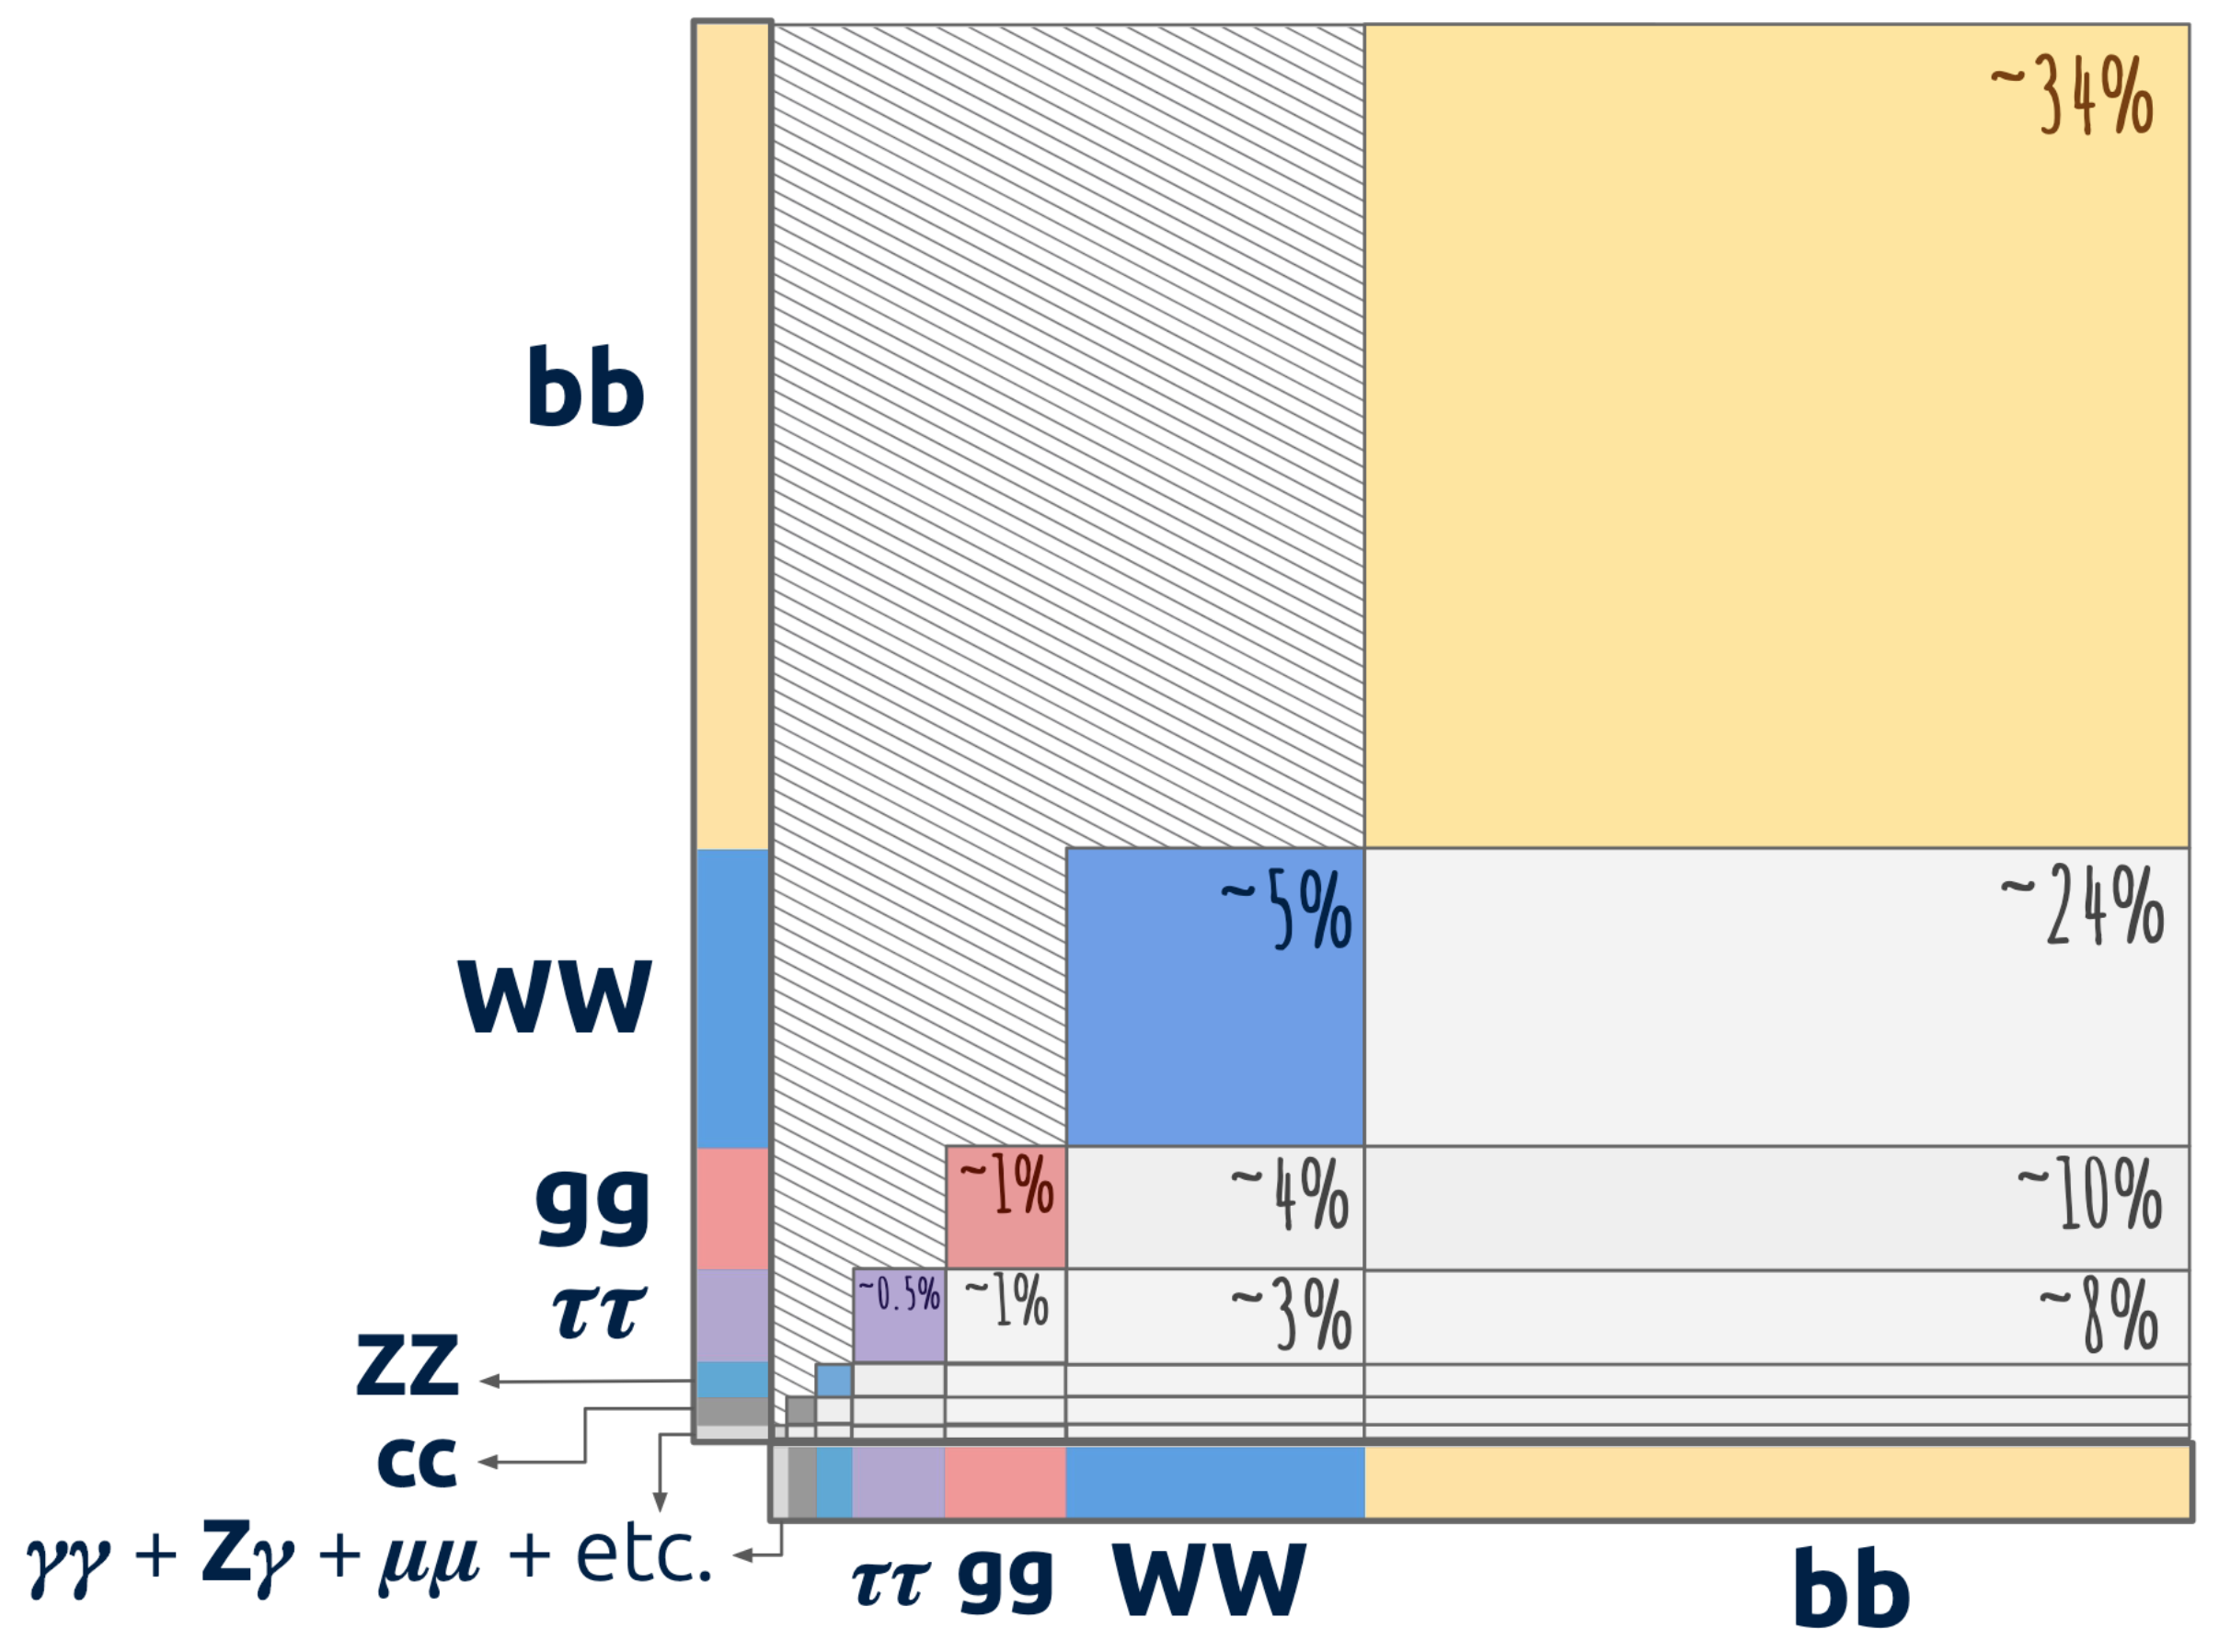
\includegraphics[width=0.7\textwidth]{branching_fraction_hh}
    \caption[]{Contributions of final states represented by area for a pair of Higgs \citep{Abbott:2708599}}
    \label{fig:branching_fraction_hh}
\end{figure}
Figure \ref{fig:branching_fraction_hh} reveals that an interesting channel is the final state with the largest branching fraction of about \qty[]{34}{percent} consisting of four $b$-quarks. However as this a fully hadronic final state it comes with the challenge of large \ac{qcd} backgrounds.

This work focuses on the boosted topology of highly energetic jets which do not allow reconstruction of $b$-jets individually but rather of final states consisting of two collimated $b$-jets inside a larger jet. The advantage of this selection is that it reduces greatly the \ac{qcd} backgrounds since highly energetic jets aare more likely to come from heavy particles such as $b$ quarks. Furthermore it is easy to trigger on events containing jets with large \pt. Although they represent a comparatively clean signal such events are rare and therefore have limited statistical power. For this reason other search strategies are better suited for the discovery of the Higgs pair production process but actual the power of this analysis lies in proving the existence of the \ktwov couplings within the \ac{sm} to which it is directly sensitive.




\section{$X\rightarrow bb$ tagger}

This work focuses on the boosted regime of the 4 $b$-quark final state. If jets are very boosted two $b$-jets can overlap and are reconstruct as variable radius jets inside a larger jet.
as explained in section \ref{sec:vr_jets}.

xbb tagger citation
\citep{ATL-PHYS-PUB-2020-019}

modeling

\section{Analysis Strategy}